\newpage

\section{Konstruktion}

Hier wird die praktische Umsetzung der Equilibrium Propagation in einer Simulationsumgebung beschrieben. Das \ac{hnn} wird als Grundlage für das Modell übernommen und in Simulink abgebildet. Darauf aufbauend werden die notwendigen Anpassungen zur Implementierung des \ac{ep} vorgenommen, insbesondere durch die Integration der Kostenfunktion und der Lernregel. Es folgt eine detaillierte Beschreibung der Simulationen des Netzwerks, einschließlich der Evaluierung der Fixpunkte und der Stabilität der Implementierung. Durch diesen Ansatz wird die Übertragbarkeit des Algorithmus auf analoge Systeme überprüft und eine Grundlage für die anschließende Analyse der Ergebnisse geschaffen.

\subsubsection{Simulationsumgebung}

\subsubsection{Übernahme des Hopfield-Netzwerks}
\label{chap:Übernahme des Hopfield-Netzwerks}

Im Folgenden soll die von \citeauthor{Scellier2017} vorgestellte Dynamik \(\frac{ds}{dt}\) eines \gls{hopfieldnetzwerk} (wie bereits im Kapitel \ref{chap:Theoretische Anwendung am Beispiel eines Hopfield-Netzwerks} gezeigt) in Simulink implementiert werden.

Um die Zustandsvariablen \(s\) darzustellen, können Integratoren genutzt werden, welche standardmäßig über Zeit integrieren. Über die Initialwerte dieser Integratoren wird die Eingabe in das \gls{hopfieldnetzwerk} definiert, welche dann über die Dynamik zu einem Fixpunkt gelangen:

\[\frac{ds}{dt}=-\frac{\partial{E}}{\partial{s}}-\beta\frac{\partial{C}}{\partial{s}}\]

Um diesen Term abzubilden werden die Gewichtungen benötigt, diese und ihre Initialwerte werden vorerst über Konstanten implementiert. Das hier untersuchte Netzwerk soll im Wertebereich \([0; 1]\) arbeiten, da sich dieser für die Anwendung auf analogen Computern eignet und für \zb Bildverarbeitung mit \(0\) für Schwarz bzw. \(1\) für Weiß genutzt werden kann. Als Aktivierungsfunktion kommt daher eine Sigmoidfunktion, die logistische Funktion \(\rho(x)=\frac{1}{1+e^{-x}}\), zum Einsatz, welche diesen Wertebereich ausgibt. Diese Funktion kann praktisch über einen Funktionsgenerator und in Simulink über einen Matlab-Funktionsblock (Siehe Anhang \ref{Anhang}) erzeugt werden. Zusätzlich zur Aktivierungsfunktion wird auch ihre Ableitung \(\rho'(x)=\rho(x)(1-\rho(x))\) benötigt, welche auf selbe Weise implementiert wird.

Diese Komponenten, die Zustände, Gewichtungen (und Bias) und die Aktivierungsfunktion werden nun gemäß der Formel \ref{Formel} mit Summierern und Multiplizierern miteinander verschaltet. Ein solches Netzwerk mit zwei Neuronen ist im Anhang \ref{Anhang} zu sehen. Die gezeigte Schaltung implementiert noch nicht die Kostenfunktion, erreicht aber bereits mit zwei Neuronen eine hohe Komplexität. Ein Netzwerk mit drei Neuronen, welches zusätzlich die Kostenfunktion implementiert ist im Anhang \ref{Anhang} dargestellt, wobei der Bias zur Übersichtlichkeit weggelassen wurde. Aus dieser Schaltung wird ersichtlich, dass die Implementierung eines \gls{hopfieldnetzwerk} mit analogen Rechenelementen bereits mit wenigen Neuronen sehr komplex und unübersichtlich wird, weshalb im Weiteren von Vektoren und Matrizen innerhalb von Simulink Gebrauch gemacht wird, siehe Anhang \ref{Anhang}. Durch die Eingabe verschieden großer Vektoren in den "`Training"'-Block, kann so die Anzahl der Neuronen des Netzwerks geändert werden. Diese Implementierung bietet potenziell auch die Möglichkeit, Trainingsdaten dynamisch aus der Matlab-Umgebung zu laden.


\paragraph{Notwendige Modifikationen am Netzwerk für Equilibrium Propagation}


\subsubsection{Simulation des angepassten Netzwerks}
\label{chap:Simulation des angepassten Netzwerks}

Im Folgenden werden einige Simulationen des in Simulink implementierten \gls{hopfieldnetzwerk} beschrieben, ein Beweis für die korrekte Funktionsweise des Netzwerkes ist im Anhang \ref{Anhang} zu finden. Die Gewichtungen werden einmalig zufällig generiert und mit diesen Werten in allen weiteren Simulationen weitergearbeitet. Es sollen also keine sinnvollen Anwendungen getestet, sondern ausschließlich die Formen der Ausgaben überprüft werden.

Die erste Simulation wird mit \(\beta=0\) und \(\vec{d}=(1,1,1)\) durchgeführt. Der Vektor \(\vec{d}\) steht dabei für die Eingabe in das Netzwerk bzw. die erwartete Ausgabe. Die Gewichtungen werden mit \((-1.21,1.319,0.3204)\) zufällig erzeugt. Wie in Abbildung \ref{Simulation HNN 1} zu sehen, gibt das Netzwerk zu Beginn der Simulation für alle Zustände einen Wert zwischen \(0.7\) und \(0.75\) aus, da für alle Zustände der Initialwert \(1\) gesetzt wurde und \(\rho(1)\approx{0.7311}\) gilt. Das Netzwerk findet einen Fixpunkt bei \(y\approx{(0.51,0.47,0.55)}\), bei dem auch die Energiefunktion ihren niedrigsten Wert erreicht. Die Kostenfunktion steigt proportional zur Energiefunktion, da sich die Ausgabe des Modells immer weiter von der Eingabe \(\vec{d}=(1,1,1)\) entfernt.

\begin{figure}[h]
  \centering
  \begin{subfigure}[b]{0.32\textwidth}
    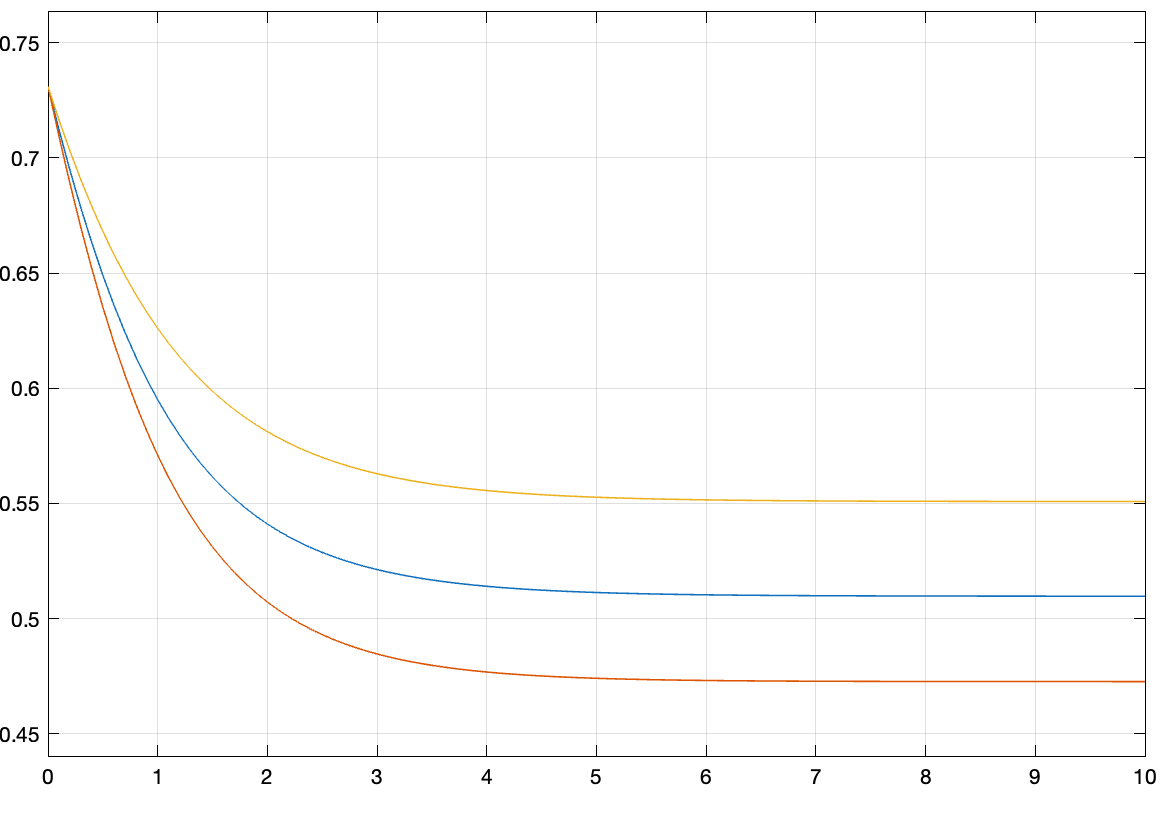
\includegraphics[width=\textwidth]{abbildungen/hnn_simulation_1_ausgabe.png}
    \caption{Ausgabe}
  \end{subfigure}%
  \hfill
  \begin{subfigure}[b]{0.32\textwidth}
    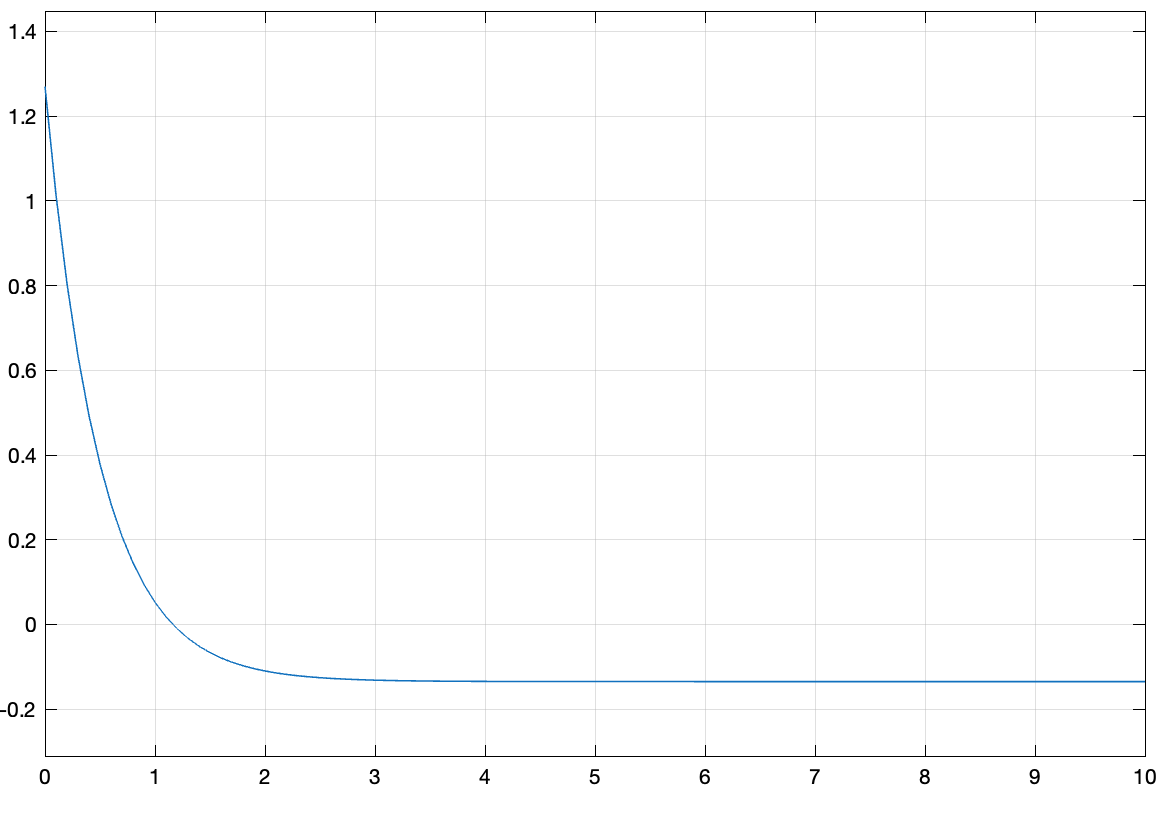
\includegraphics[width=\textwidth]{abbildungen/hnn_simulation_1_energiefunktion.png}
    \caption{Energie}
  \end{subfigure}%
  \hfill
  \begin{subfigure}[b]{0.32\textwidth}
    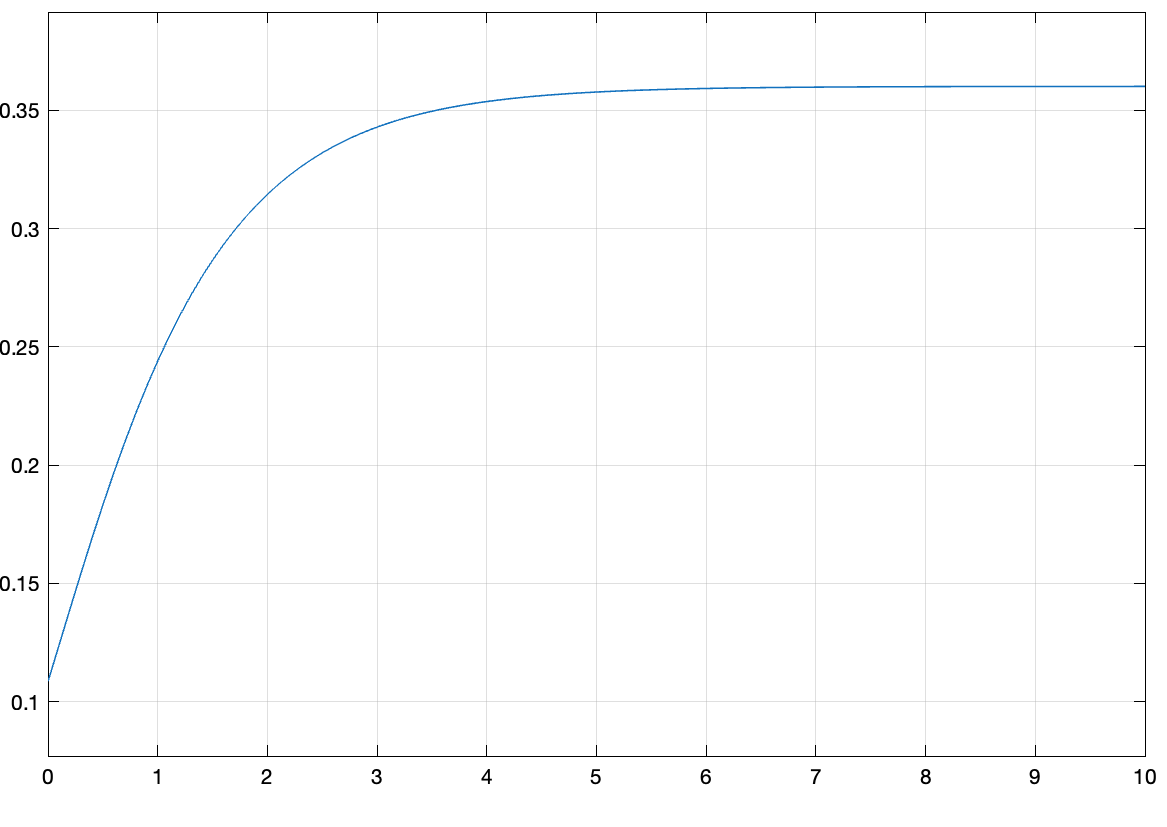
\includegraphics[width=\textwidth]{abbildungen/hnn_simulation_1_kostenfunktion.png}
    \caption{Kosten}
  \end{subfigure}
  \caption{Erste Simulation des \gls{hopfieldnetzwerk}. Quelle: \textit{Eigene Darstellung}}
  \label{fig:Simulation HNN 1}
\end{figure}

Für die zweite Simulation wird die Eingabe zu \(\vec{d}=(1,0,0)\) geändert. Da das \gls{hopfieldnetzwerk} die Eigenschaften eines assoziativen Speichers besitzt (vgl. Kapitel \ref{chap:Das Hopfield-Netzwerk: Eine Herangehensweise an neuronale Netze}), ist zu erwarten, dass das Netzwerk die gleiche Ausgabe wie aus der vorherigen Simulation liefert. Diese These lässt sich anhand der Abbildung \ref{fig:Simulation HNN 2} bestätigen.

\begin{figure}[h]
  \centering
  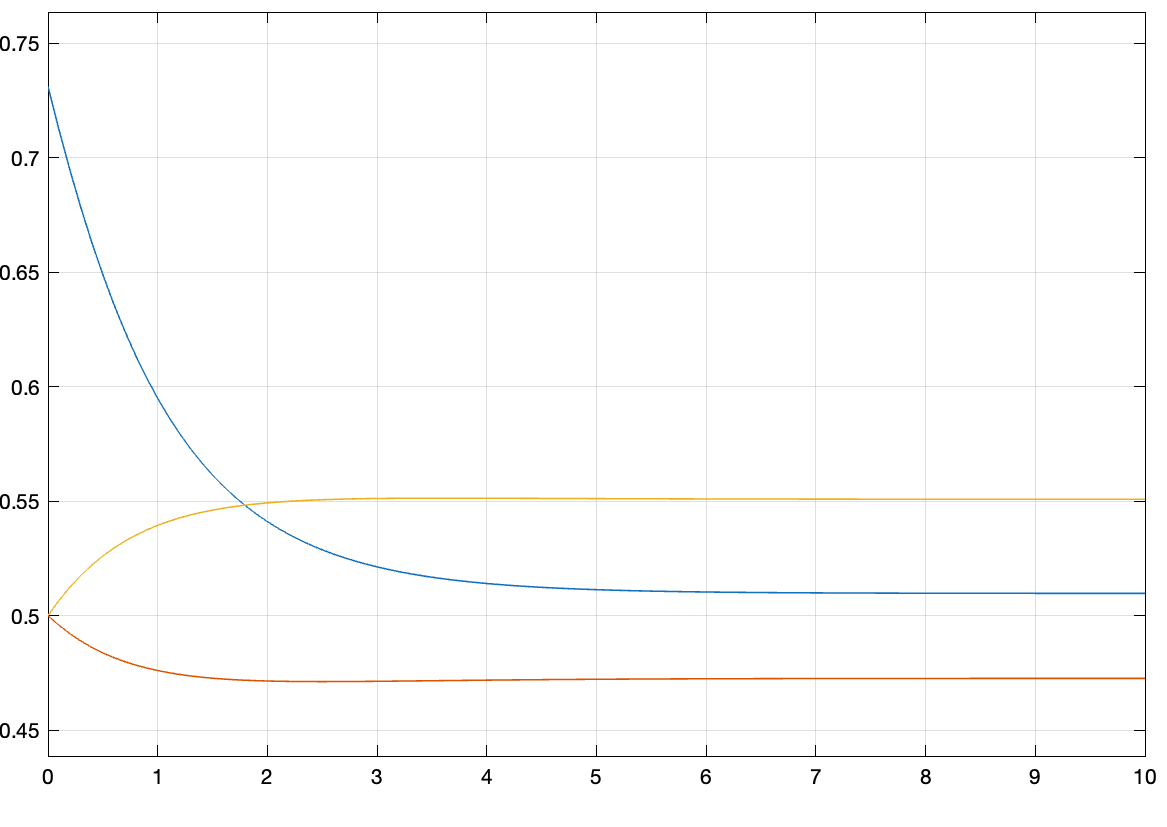
\includegraphics[width=0.5\textwidth]{abbildungen/hnn_simulation_2_ausgabe.png}
  \caption{Zweite Simulation des \gls{hopfieldnetzwerk}. Quelle: \textit{Eigene Darstellung}}
  \label{fig:Simulation HNN 2}
\end{figure}

Die dritte Simulation wird mit \(\beta=1\) durchgeführt, wodurch die Zustände des Netzwerks höhere Werte annehmen und somit die Kostenfunktion kleiner sein sollte. Dementsprechend sollte die Energiefunktion auch einen höheren Wert annehmen, da die Ausgabe des Netzwerks vom optimalen Ergebnis aus der ersten Simulation abweicht. Die Ergebnisse der Simulation aus Abbildung \ref{fig:Simulation HNN 3} bestätigen diese Annahmen.

\begin{figure}[h]
  \centering
  \begin{subfigure}[b]{0.32\textwidth}
    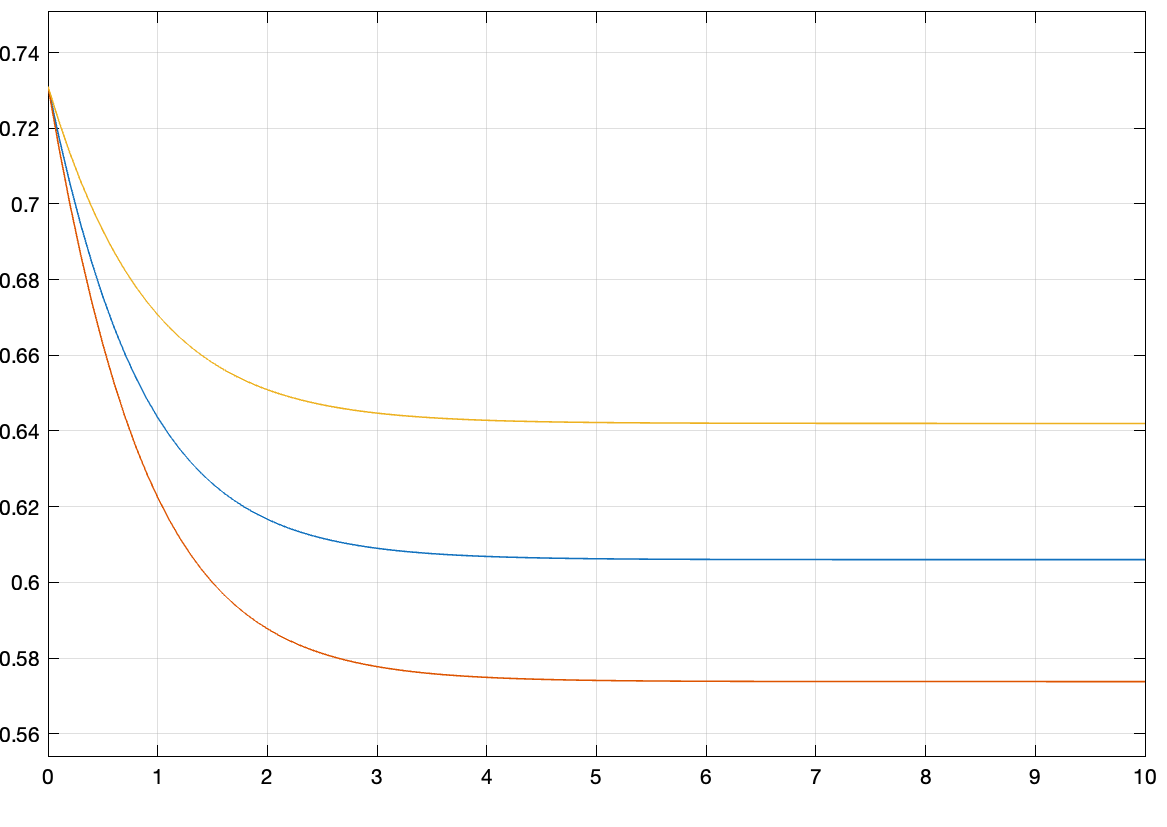
\includegraphics[width=\textwidth]{abbildungen/hnn_simulation_3_ausgabe.png}
    \caption{Ausgabe}
  \end{subfigure}%
  \hfill
  \begin{subfigure}[b]{0.32\textwidth}
    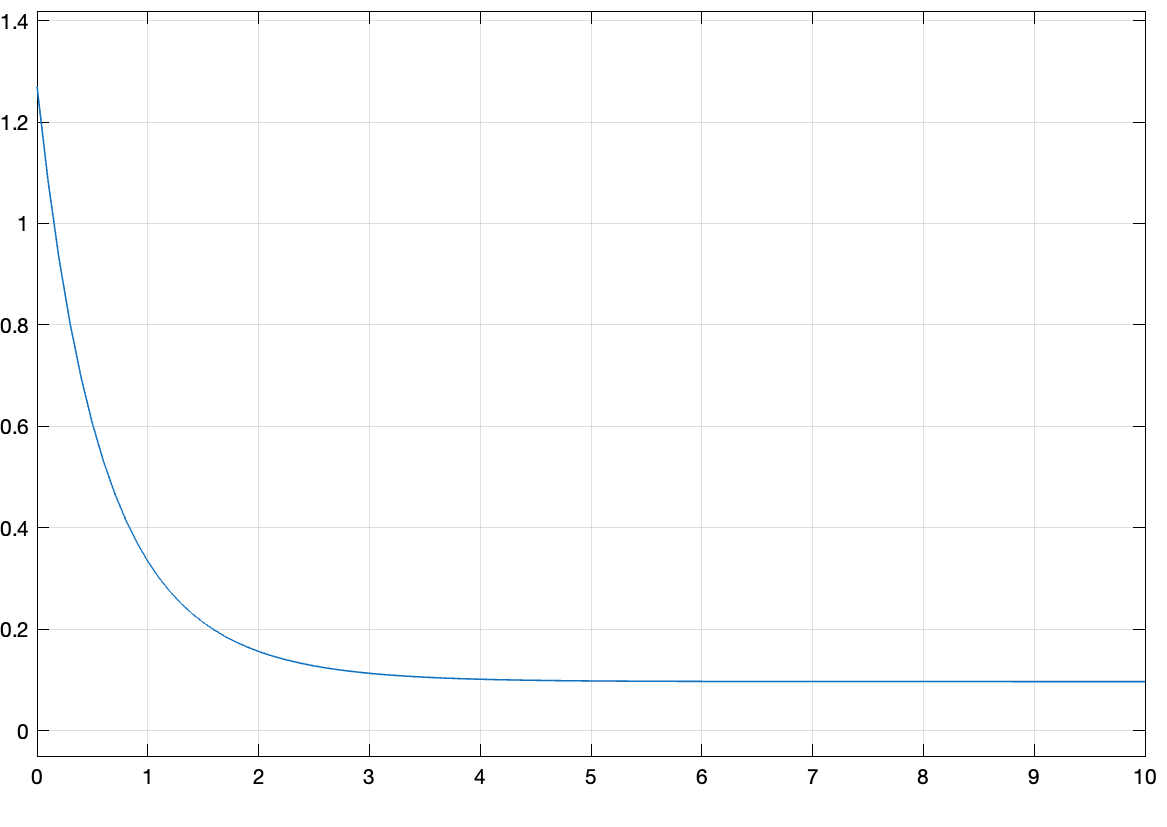
\includegraphics[width=\textwidth]{abbildungen/hnn_simulation_3_energiefunktion.png}
    \caption{Energie}
  \end{subfigure}%
  \hfill
  \begin{subfigure}[b]{0.32\textwidth}
    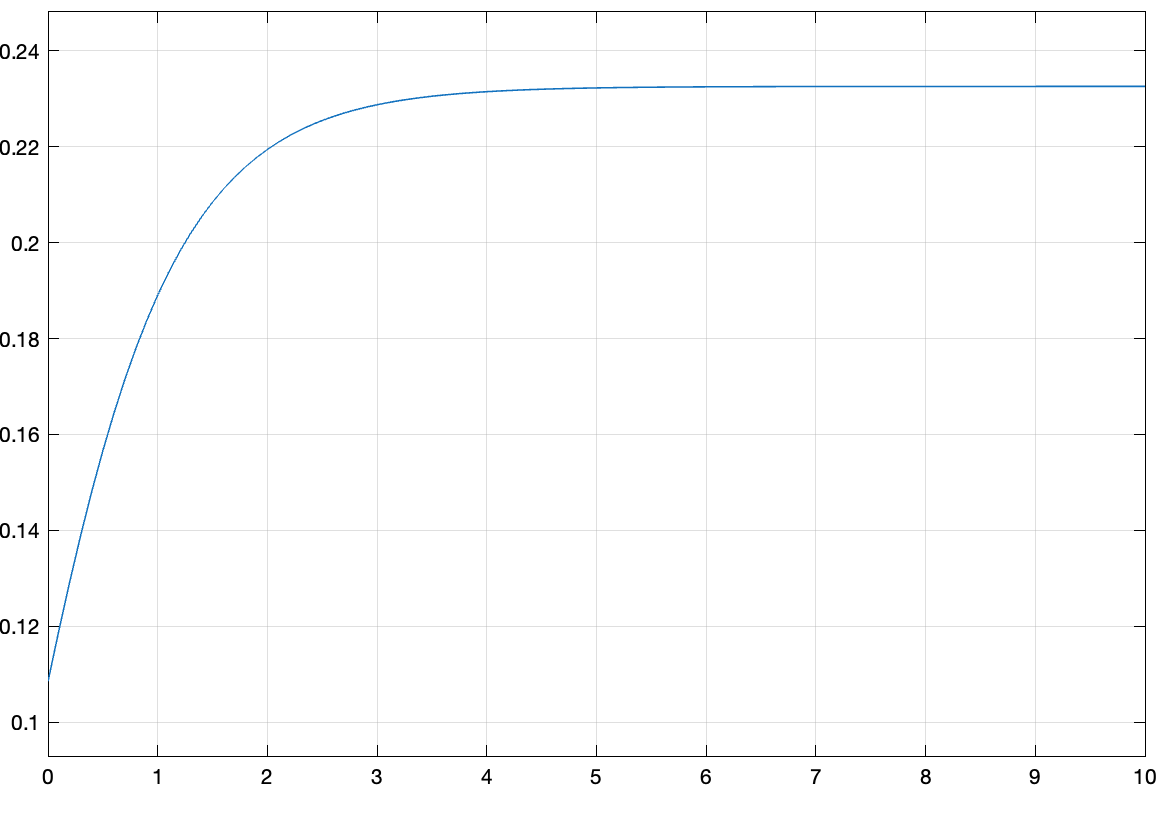
\includegraphics[width=\textwidth]{abbildungen/hnn_simulation_3_kostenfunktion.png}
    \caption{Kosten}
  \end{subfigure}
  \caption{Dritte Simulation des \gls{hopfieldnetzwerk}. Quelle: \textit{Eigene Darstellung}}
  \label{fig:Simulation HNN 3}
\end{figure}


\subsubsection{Konstruktion des Equilibrium Propagation Algorithmus}

\paragraph{Umsetzung der theoretischen Modelle in der Simulationssoftware}


\subsubsection{Anwendung auf das Hopfield-Netzwerk}


\subsubsection{Herausforderungen bei der Übernahme und Anpassung}
\label{chap:Herausforderungen bei der Übernahme und Anpassung}

Eine Herausforderung bei der Umsetzung des \gls{c-ep} ist das Finden einer passenden Aktivierungsfunktion für die Zusammenarbeit mit der Lernregel \(\frac{dW_{ij}}{dt}\) und einer passenden Lernrate \(\eta\), welche eine effiziente Konvergenz der Gewichtungen gewährleistet. Für die bisher gewählte Aktivierungsfunktion, die logistische Funktion wie dargestellt in Abbildung \ref{fig:Graph der Aktivierungsfunktion}, gilt \(\rho(x) > 0\), weshalb auch die Lernregel immer positiv ist. Die Auswirkungen dessen sind in Abbildung \ref{fig:C-EP Non-Negative Aktivierungsfunktion} dargestellt, wobei als Zielwert für das Netzwerk \(\vec{d}=(0,0,0)\) gewählt wurde. Die Ausgabe des Netzwerks richtet sich zu Beginn der zweiten Phase offensichtlich in Richtung der Zielwerte, steigt aber nach einer kurzen Zeit stetig an, da der positive Einfluss der Gewichtungen den negativen der Kostenfunktion übersteigt.

\begin{figure}[h]
  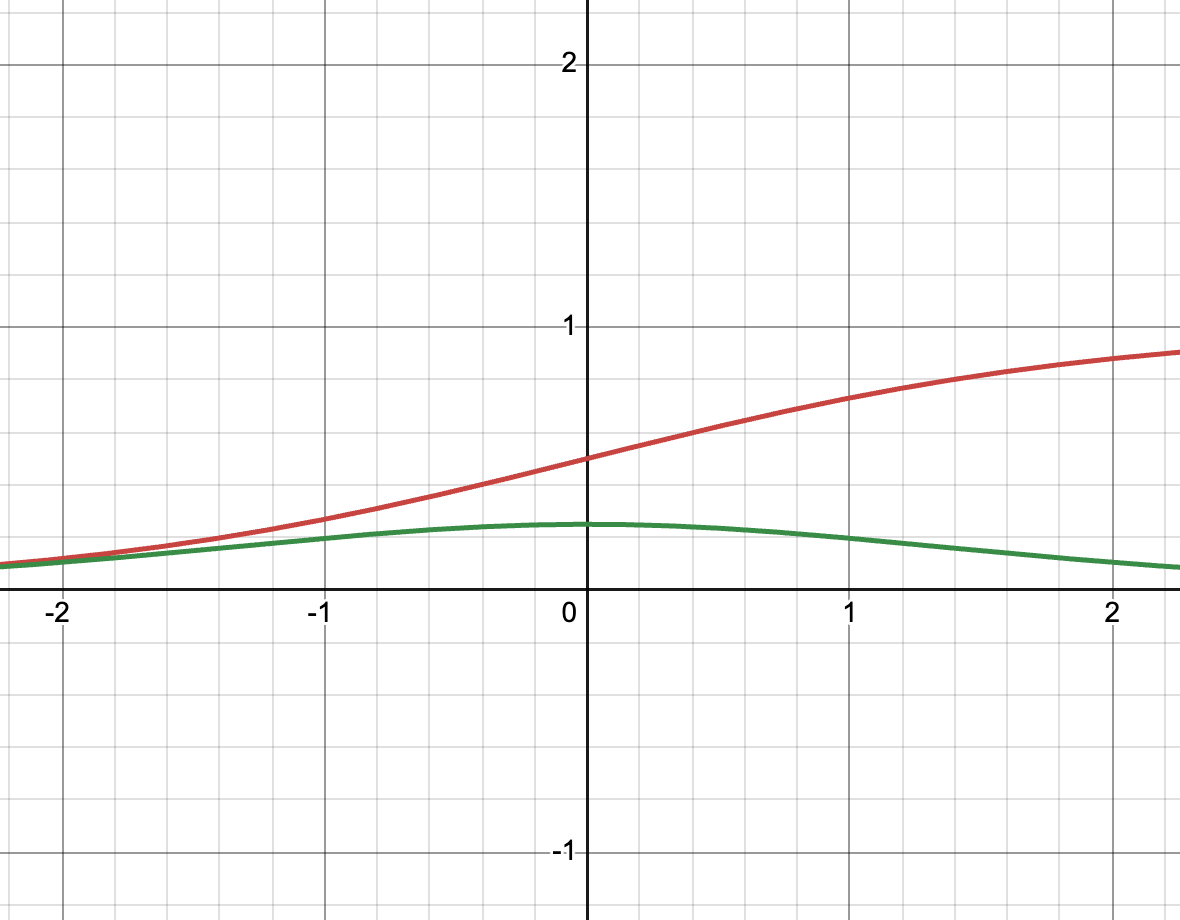
\includegraphics[width=0.5\textwidth]{abbildungen/sigmoid_funktion.png}
  \caption{Graph der Aktivierungsfunktion \(\rho(x)=\frac{1}{1+e^{-x}}\) (rot) und ihrer Ableitung (grün). Quelle: \textit{Eigene Darstellung}}
  \label{fig:Graph der Aktivierungsfunktion}
\end{figure}

\begin{figure}[h]
  \centering
  \begin{subfigure}[b]{0.5\textwidth}
    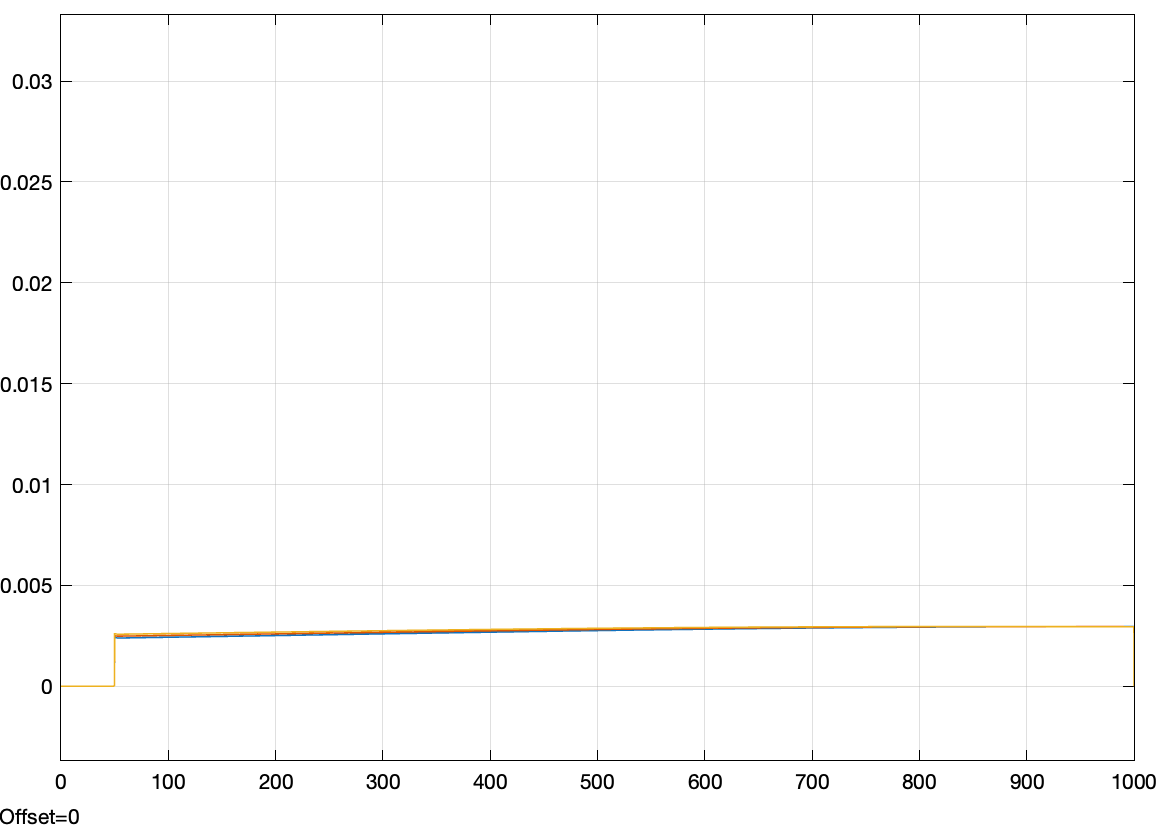
\includegraphics[width=\textwidth]{abbildungen/c_ep_non_negative_activation_weight_update.png}
    \caption{Änderungsrate der Gewichtungen}
  \end{subfigure}%
  \hfill
  \begin{subfigure}[b]{0.5\textwidth}
    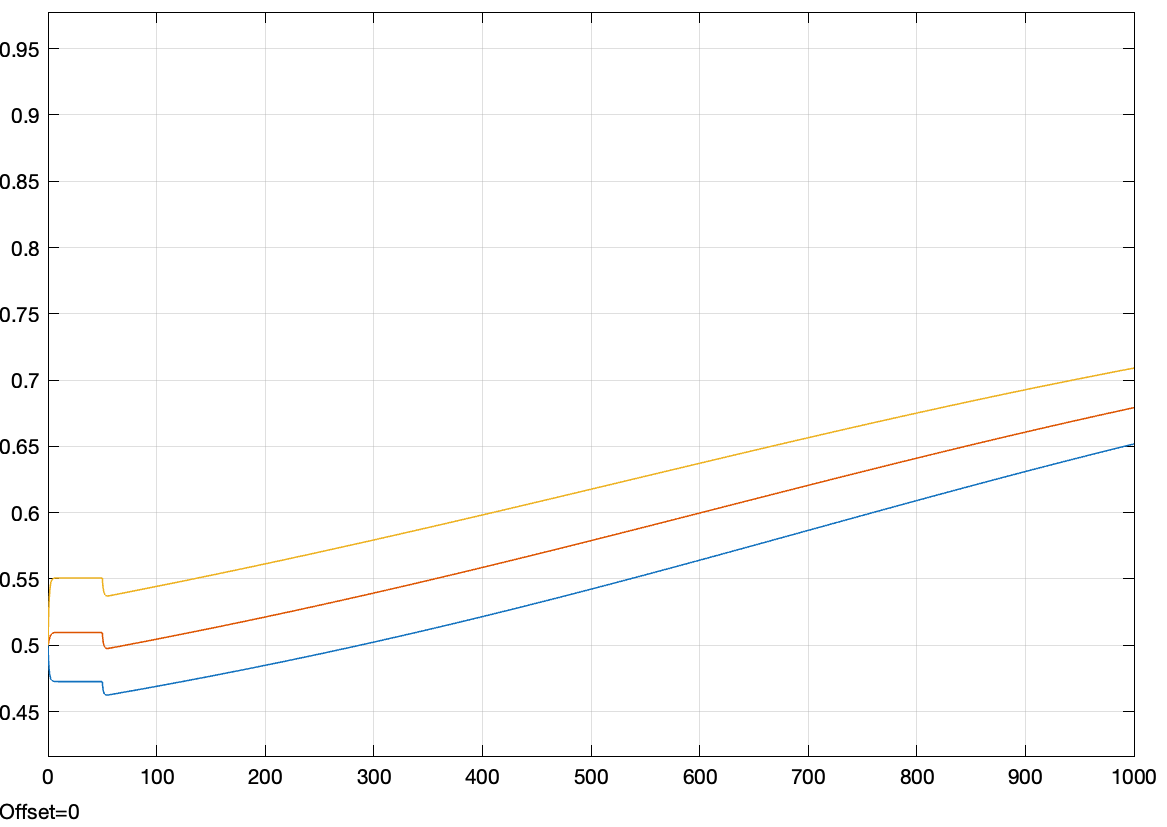
\includegraphics[width=\textwidth]{abbildungen/c_ep_non_negative_activation_ausgabe.png}
    \caption{Ausgabe des Modells}
  \end{subfigure}
  \caption{Auswirkungen einer nicht-negativen Aktivierungsfunktion auf das \gls{c-ep}. Quelle: \textit{Eigene Darstellung}}
  \label{fig:C-EP Non-Negative Aktivierungsfunktion}
\end{figure}

Die Dauer der beiden Phasen des \gls{c-ep} wurde durch die Konvergenz dieser definiert. So soll die erste Phase durchgeführt werden bis das Netzwerk einen Fixpunkt findet, für die zweite Phase müssen Fixpunkte des Netzwerkes und der Parameter gefunden werden \cite[vgl. S. 3]{Ernoult2020}. Die Bestimmung sinnvoller Werte für die Dauer dieser Phasen stellt die Umsetzung des Lernprozesses vor eine weitere Herausforderung. Wie bereits in \ref{chap:Simulation des angepassten Netzwerks} gezeigt, propagiert das implementierte \gls{hopfieldnetzwerk} mit beliebigem \(\beta\) zuverlässig innerhalb von weniger als zehn Zeiteinheiten zu einem Fixpunkt. Gleiches sollte auf die feste Phase zutreffen, dies ist aber, wie in Abbildung \ref{fig:C-EP Konvergenz Problem} gezeigt, nicht der Fall. Eine mögliche Ursache hierfür stellt erneut die Auswahl der Aktivierungsfunktion dar, da, wie aus Abbildung \ref{fig:Graph der Aktivierungsfunktion} abzulesen, \(\rho(x) > 0\) bzw. \(\dot{\rho}(x) > 0\) und somit \(\frac{dW_{ij}}{dt} > 0\) gilt. Eine Simulation mit \(\vec{d}=(0.8,0.8,0.8)\) und \(\eta=0.1\) zeigt die valide Anpassung der Gewichtungen bis zu einem Zeitpunkt \(t\approx250\) aber die anschließende fehlende Konvergenz der Parameter.

\begin{figure}[h]
  \centering
  \begin{subfigure}[b]{0.3\textwidth}
    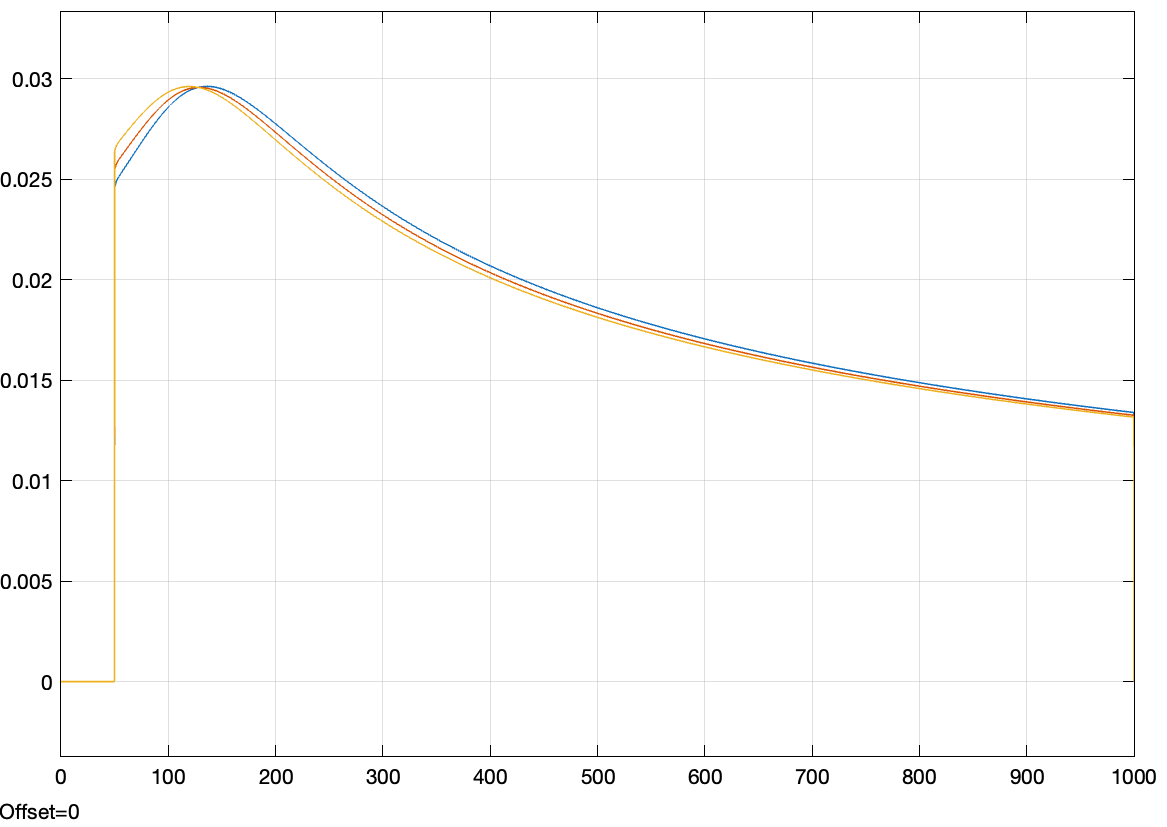
\includegraphics[width=\textwidth]{abbildungen/c_ep_convergence_weight_update.png}
    \caption{Änderungsrate der Gewichtungen}
  \end{subfigure}%
  \hfill
  \begin{subfigure}[b]{0.3\textwidth}
    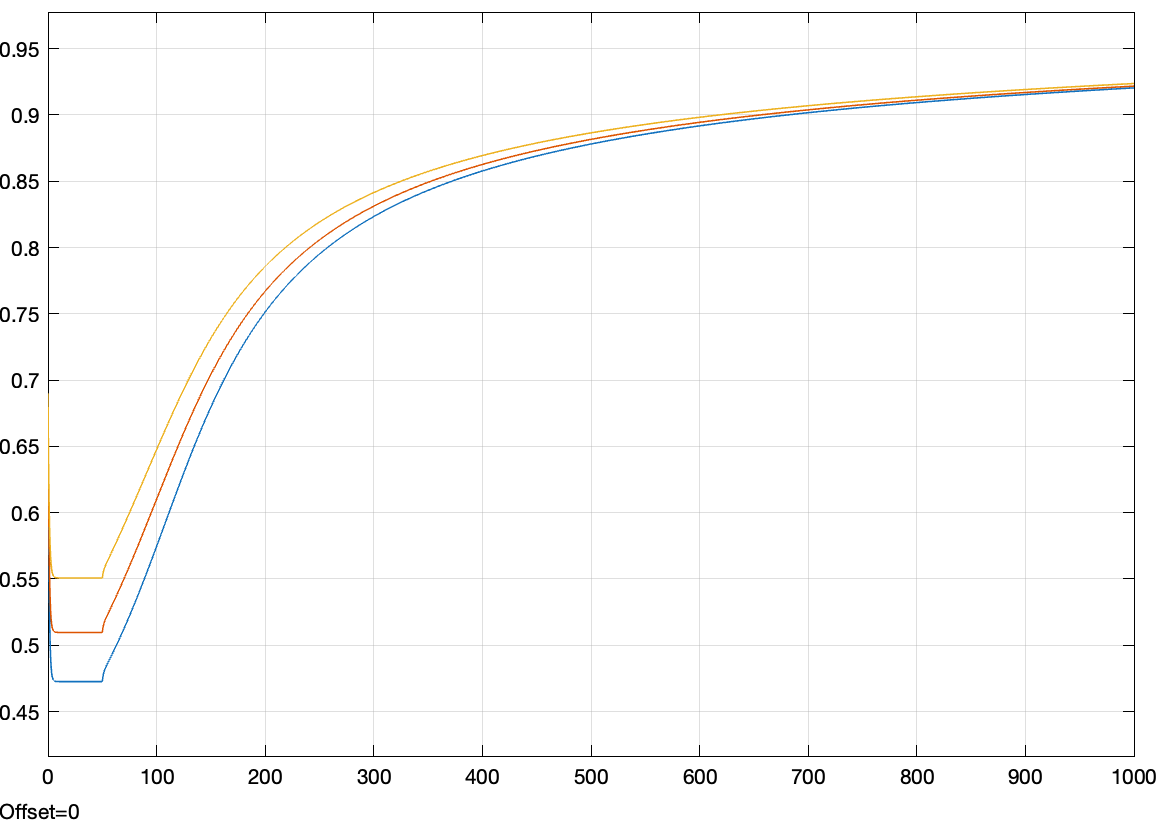
\includegraphics[width=\textwidth]{abbildungen/c_ep_convergence_ausgabe.png}
    \caption{Ausgabe des Modells}
  \end{subfigure}%
  \hfill
  \begin{subfigure}[b]{0.3\textwidth}
    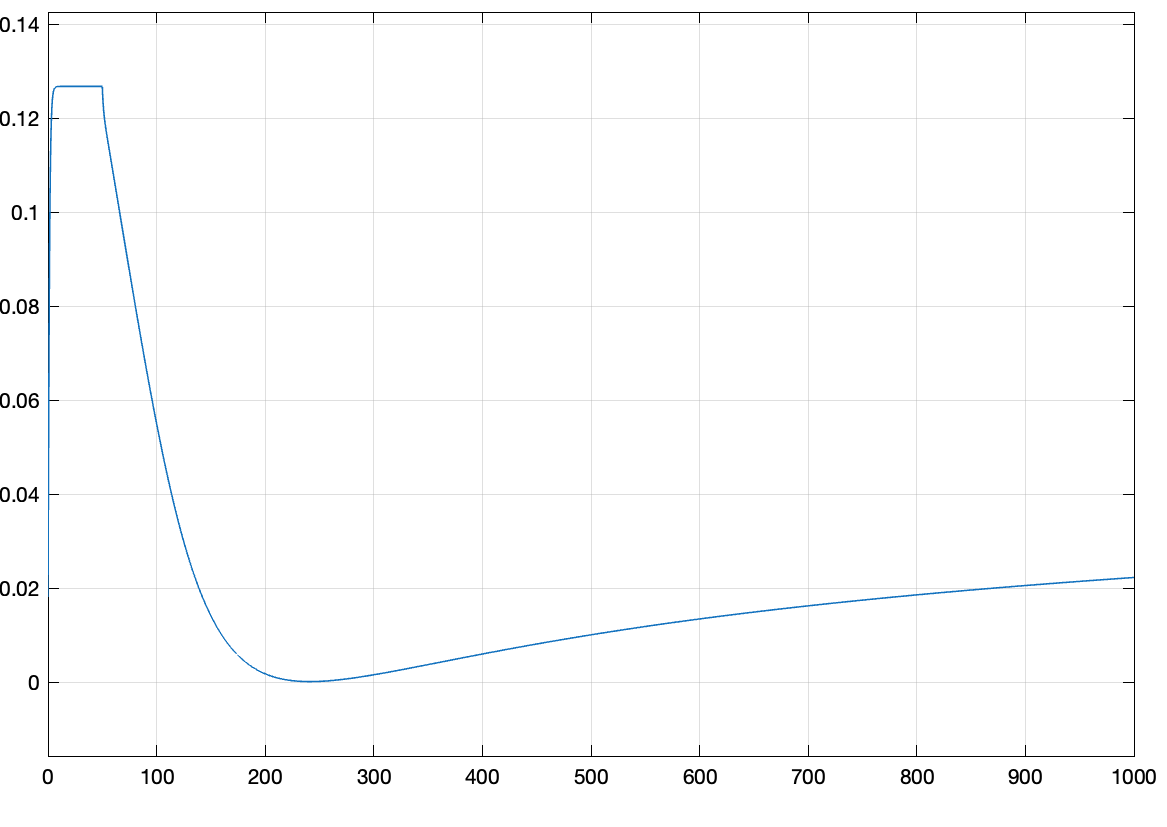
\includegraphics[width=\textwidth]{abbildungen/c_ep_convergence_kosten.png}
    \caption{Kosten des Modells}
  \end{subfigure}
  \caption{Die Parameter des Modells gelangen zu keinem Fixpunkt und verfehlen damit das Minimum der Kostenfunktion. Quelle: \textit{Eigene Darstellung}}
  \label{fig:C-EP Konvergenz Problem}
\end{figure}

Um Fehler bei der Auswahl der Aktivierungsfunktion oder der Übernahme der Lernregel auszuschließen, wird im Folgenden die von \citeauthor{Ernoult2020} ursprünglich für \gls{c-ep} vorgestellte Lernregel verwendet:

\[\Delta^{C-EP}_{Wnn+1}(\beta,\eta,t)=\frac{1}{\beta}\left(\sigma\left(s^{n,\beta,\eta}_{t+1}\right)\sigma\left(s^{n+1,\beta,\eta}_{t+1}\right)^\intercal-\sigma\left(s^{n,\beta,\eta}_{t}\right)\sigma\left(s^{n+1,\beta,\eta}_{t}\right)^\intercal\right)\]

Angewandt auf das hier genutzte \gls{hopfieldnetzwerk} und unter Beachtung der Lernrate \(\eta\) ergibt sich:

\[\Delta^{C-EP}_{W_{ij}}(\eta,t)\propto\eta\left(\rho(u^{\beta}_{t+1,i})\rho(u^{\beta}_{t+1,j})-\rho(u^{\beta}_{t,i})\rho(u^{\beta}_{t,j})\right)\]

\[\Delta^{C-EP}_{b_{i}}(\eta,t)\propto\eta\left(\rho(u^{\beta}_{t+1,i})-\rho(u^{\beta}_{t,i})\right)\]

Anhand dieser Lernregel kann die Dynamik \(\frac{dW_{ij}}{dt}\) approximiert werden, indem praktisch mit einer Zeitverschiebung gearbeitet wird. Simulink bietet hierfür den Block "`Transport Delay"', welcher ein kontinuierliches Eingangssignal um einen beliebigen Zeitraum verschiebt. Die Zeitverschiebung ist kein grundlegender Bestandteil herkömmlicher analoger Computer (siehe Kapitel \ref{chap:Typische Komponenten und Bauweisen analoger Computer}) und für diese Aufgabe eignet sich auch wieder ein hybrider Ansatz, da Informationen (auch wenn nur über einen sehr kurzen Zeitraum) gespeichert werden müssen. Es existieren aber auch Ansätze zur Annäherung einer Zeitverschiebung auf analoger Hardware \cite[vgl. S. 117 ff.]{Ulmann2022}. Negative Gewichtsanpassungen sind mit diesem Ansatz ohne weiteres möglich und der beispielhafte Durchlauf des Netzwerks mit \(\vec{d}=(0.8,0.8,0.8)\) (jetzt mit \(\eta=10\)) konvergiert mit diesem Ansatz zu sinnvollen Gewichten (siehe Abbildung \ref{fig:C-EP Annäherung Konvergenz}). Im Anhang \ref{Anhang} wird das Simulink-Modell zu diesem Ansatz gezeigt.

\begin{figure}[h]
  \centering
  \begin{subfigure}[b]{0.3\textwidth}
    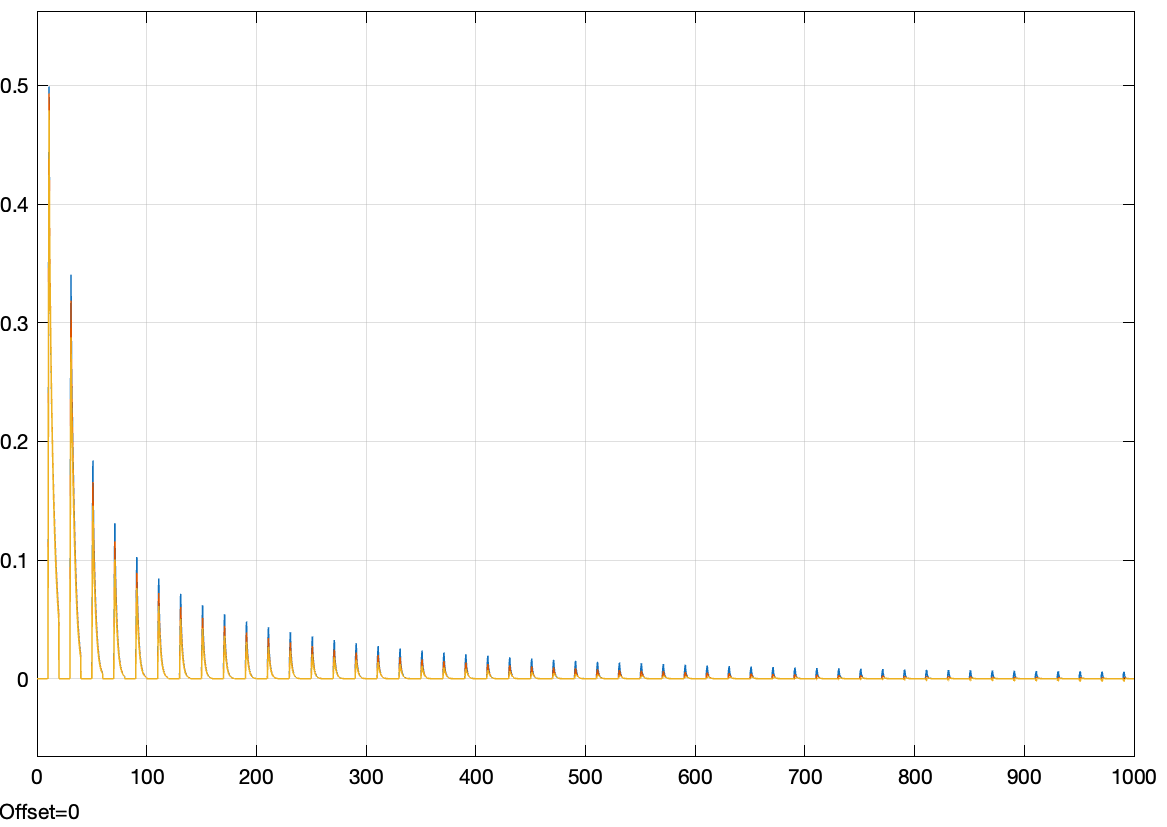
\includegraphics[width=\textwidth]{abbildungen/c_ep_approx_convergence_weight_update.png}
    \caption{Änderungsrate der Gewichtungen}
  \end{subfigure}%
  \hfill
  \begin{subfigure}[b]{0.3\textwidth}
    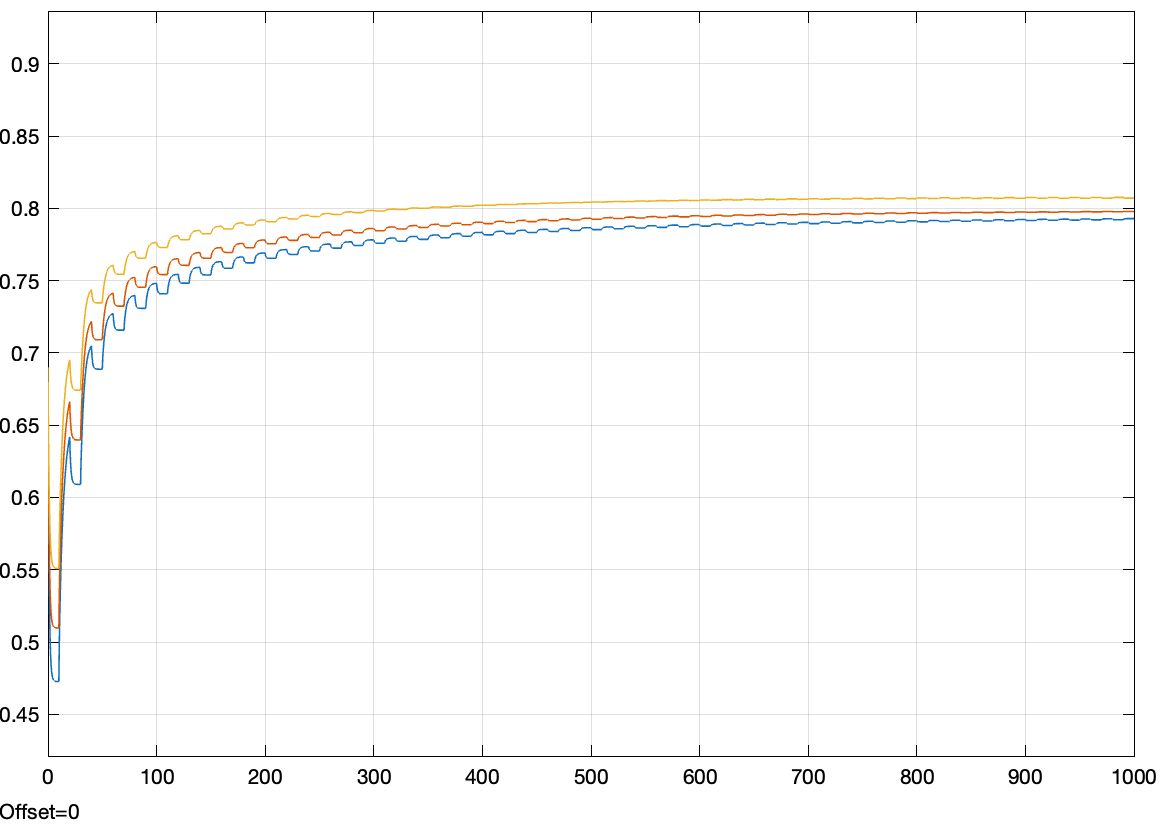
\includegraphics[width=\textwidth]{abbildungen/c_ep_approx_convergence_ausgabe.png}
    \caption{Ausgabe des Modells}
  \end{subfigure}%
  \hfill
  \begin{subfigure}[b]{0.3\textwidth}
    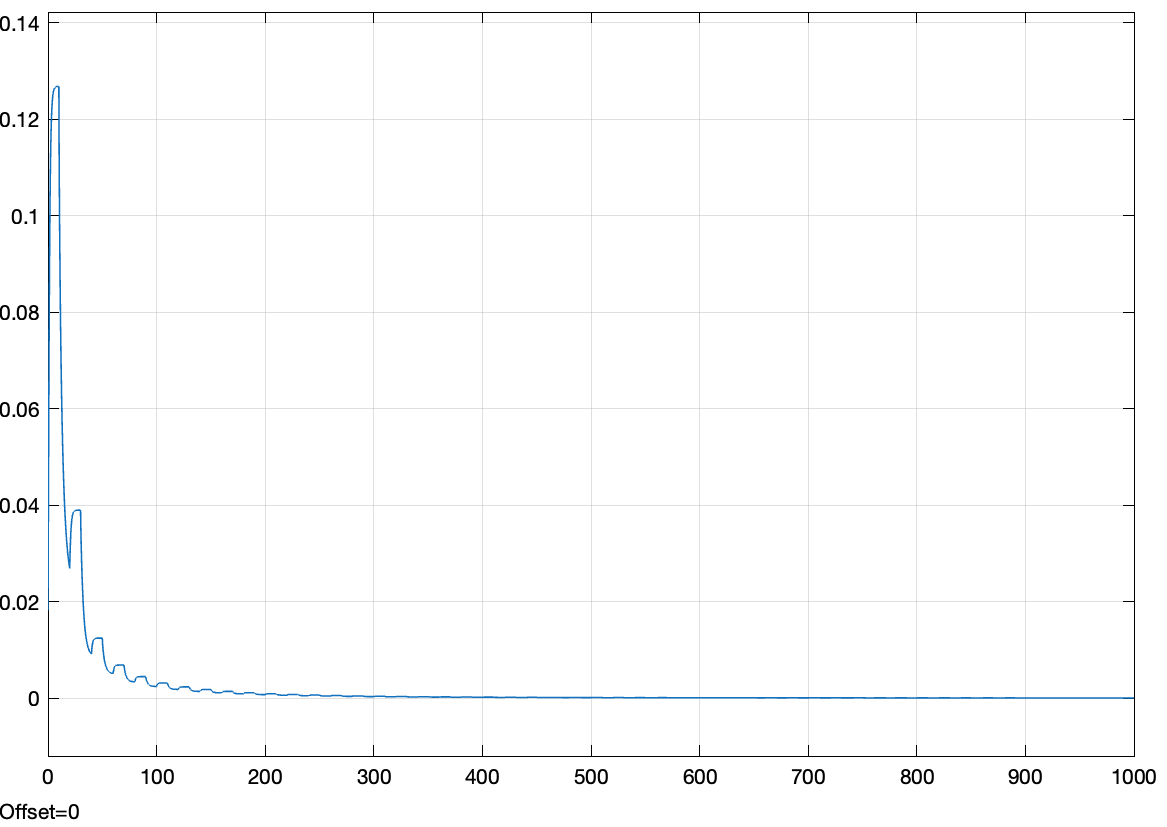
\includegraphics[width=\textwidth]{abbildungen/c_ep_approx_convergence_kosten.png}
    \caption{Kosten des Modells}
  \end{subfigure}
  \caption{Eine Annäherung an C-EP findet passende Parameter für das Netzwerk. Quelle: \textit{Eigene Darstellung}}
  \label{fig:C-EP Annäherung Konvergenz}
\end{figure}


\subsubsection{Strategien zur Fehlerbehebung und Optimierung}
\label{chap:Strategien zur Fehlerbehebung und Optimierung}

Im vorherigen Kapitel \ref{chap:Herausforderungen bei der Übernahme und Anpassung} wurde bereits gezeigt, dass die Implementierung des \ac{c-ep} sinnvolle Gewichte für \(\vec{d}=(0.8,0.8,0.8)\) findet. Da die Aktivierungsfunktion in Annäherung an \(\rho(x)=0\) bzw. \(\rho(x)=1\) eher große Werte \(x\) benötigt (\(\rho(4.5952)\approx0.99\)), müssen die Zustände des Netzwerks bzw. die Gewichte entsprechend große Werte annehmen, um die Zielwerte \(0\) bzw. \(1\) abzubilden. Die Konvergenz der Gewichte ist für diese Zielwerte auch nicht möglich, weshalb das \ac{c-ep} in diesem Fall die Gewichte endlos vergrößert bzw. verkleinert. Eine mögliche Lösung hierfür könnte das Austauschen der Aktivierungsfunktion gegen die sog. "`ReLU"'-Funktion (\(R(x)=max(x,0)\)) sein, welche linear im Wertebereich \(x>0\) verläuft. Beim Anwenden auf das \ac{hnn} führt ReLU aber zu Problemen, da das Netzwerk damit nicht konvergiert und somit unbrauchbare Werte ausgibt. In Anlehnung an \cite[vgl. S. 31]{Ernoult2020} kann die bereits genutzte Aktivierungsfunktion \(\rho(x)=\frac{1}{1+e^{-x}}\) skaliert werden, um ihre S-Kurve zu stauchen und damit die Annäherung an \(0\) bzw. \(1\) zu vereinfachen. Die abgewandelte Funktion \(\rho(x)=\frac{1}{1+e^{-4x}}\) ist in Abbildung \ref{fig:Graph der skalierten Aktivierungsfunktion} dargestellt.

\begin{figure}[h]
  \label{fig:Graph der skalierten Aktivierungsfunktion}
  \caption{Graph der Aktivierungsfunktion (rot) und der skalierten Variante \(\rho(x)=\frac{1}{1+e^{-4x}}\) (orange)}
  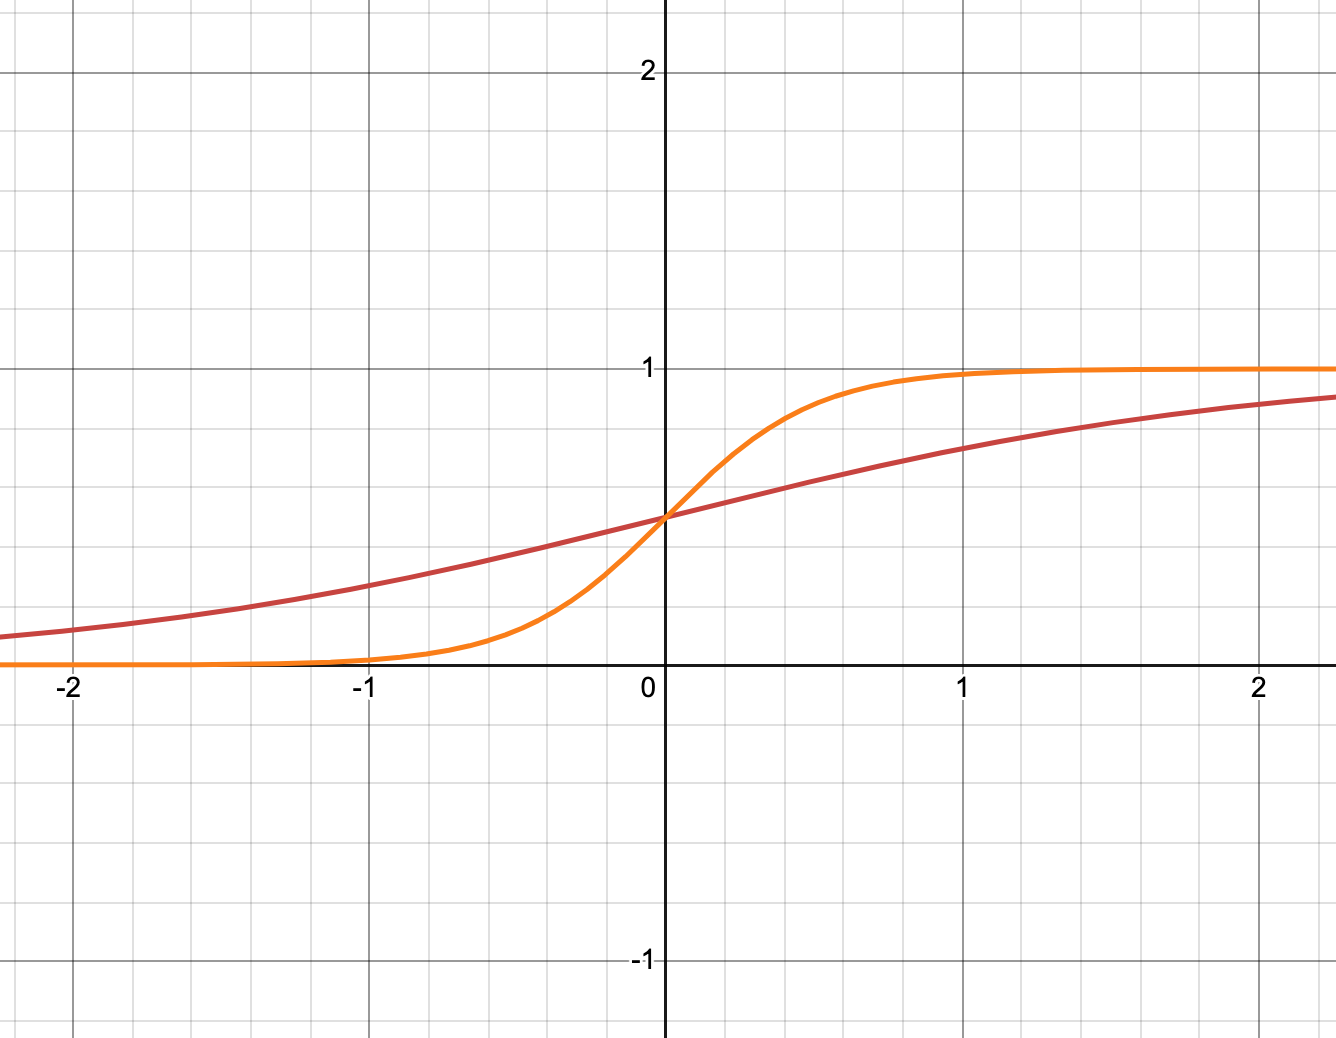
\includegraphics[width=0.5\textwidth]{abbildungen/sigmoid_funktion_skaliert.png}
  \\
  Quelle: Eigene Darstellung
\end{figure}

Mit den Parametern \(\beta=1\) und \(\eta=1\) findet das \ac{c-ep} mit dieser skalierten Aktivierungsfunktion und den Zielwerten \(\vec{d}=(0,0,0)\) Gewichte, welche die Ausgabe \(\vec{y}\approx(0.14,0.14,0.16)\) erzeugen, damit zwar in die Nähe der Zielwerte gelangen aber diese noch immer drastisch verfehlen. Werden aber Zielwerte abseits der Grenzwerte \(0\) bzw. \(1\) beispielsweise \(\vec{d}=(0.2,0.5,0.8)\) betrachtet, so werden Gewichte gefunden, mit denen ein Fehler von \(C(y)<0.001\) erreicht wird. Ein weiterer Durchlauf mit den Zielwerten \(\vec{d}=(0.3,0.4,0.7)\) führt zu einem Fehler der Größenordnung \(10^{-6}\) in unter zehn Epochen. Aufgrund dieser Verbesserungen wird mit der skalierten Aktivierungsfunktion weitergearbeitet.


\paragraph{Validierung des Algorithmus durch Testläufe}


